\section{Data Access and Execution Abstractions}
\label{sec:middleware}

The algorithmic components of the LSST Science Pipelines are built on a suite of packages that together form a powerful data access and execution framework (\texttt{pex\_config}, \texttt{resources}, \texttt{daf\_butler}, \texttt{pipe\_base}, \texttt{ctrl\_mpexec}, and \texttt{ctrl\_bps}).
Unlike most of the rest of the codebase, these packages can be individually installed with \texttt{pip} as well as EUPS and can be used on their own.

\subsection{Butler}

Early in the development of the LSST Science Pipelines software it was decided that the algorithmic code should be written without knowing where files came from, what format they were written in, where the outputs are going to be written or how they are going to be stored.
All that the algorithmic code needs to know is the relevant data model and the Python type.
To meet these requirements we developed a library called the Data Butler \citep[see e.g.,][]{2022SPIE12189E..11J,2023arXiv230303313L}.

The Butler internally is implemented as a registry, a database keeping track of datasets, and a datastore, a storage system that can map a Butler dataset to a specific collection of bytes.
A datastore is usually a file store (including POSIX file system, S3 object stores, or WebDAV) but it is also possible to store metrics directly into the Sasquatch metrics service \citep{SQR-068,2024SPIE13101E..1MF}.

\begin{deluxetable}{ll}

%% Keep a portrait orientation

%% Over-ride the default font size
%% Use Default (12pt)

%% Use \tablewidth{?pt} to over-ride the default table width.
%% If you are unhappy with the default look at the end of the
%% *.log file to see what the default was set at before adjusting
%% this value.

%% This is the title of the table.
\tablecaption{Common dimensions present in the default dimension universe.\label{tab:dims}}

%% This command over-rides LaTeX's natural table count
%% and replaces it with this number.  LaTeX will increment
%% all other tables after this table based on this number
%% \tablenum{1}

%% The \tablehead gives provides the column headers.  It
%% is currently set up so that the column labels are on the
%% top line and the units surrounded by ()s are in the
%% bottom line.  You may add more header information by writing
%% another line between these lines. For each column that requries
%% extra information be sure to include a \colhead{text} command
%% and remember to end any extra lines with \\ and include the
%% correct number of &s.
\tablehead{\colhead{Name} & \colhead{Description} \\
\colhead{} & \colhead{} }

%% All data must appear between the \startdata and \enddata commands
\startdata
\texttt{instrument} &  Instrument.  \\
\texttt{band} & Waveband of interest.  \\
\texttt{physical\_filter} &  Filter used for the exposure. \\
\texttt{day\_obs} & The observing day. \\
\texttt{group} &  Group identifier. \\
\texttt{exposure} & Individual exposure. \\
\texttt{visit} &  Collection of 1 or 2 exposures. \\
\texttt{tract} &  Tesselation of the sky. \\
\texttt{patch} &  Patch within a tract.\\
\enddata

%% Include any \tablenotetext{key}{text}, \tablerefs{ref list},
%% or \tablecomments{text} between the \enddata and
%% \end{deluxetable} commands

\end{deluxetable}

A core concept of the Butler is that every dataset must be given what we call a ``data coordinate.''
The data coordinate locates the dataset in the dimensional space where dimensions are defined in terms that scientists understand.
Some commonly used dimensions are listed in Table~\ref{tab:dims}.
Each dataset is uniquely located by specifying its dataset type, its run collection, and its coordinates, with Butler refusing to accept another dataset that matches all three of those values.
The dataset type defines the relevant dimensions (such as whether this is referring to observations or a sky map) and the associated Python type representing the dataset.
The run collection can be thought of as a folder grouping datasets created by the same batch operation, but does not have to be a folder within a file system.

As a concrete example, the file from one detector of an LSSTCam observation taken sometime in 2025 could have a data coordinate of \texttt{instrument="LSSTCam", detector=42, exposure=2025080300100} and be associated with a \texttt{raw} dataset type.
The \texttt{exposure} record itself implies other information such as the physical filter and the time of observation.
A deep coadd on a patch of sky would not have \texttt{exposure} dimensions at all and would instead be something like \texttt{instrument="LSSTCam", tract=105, patch=2, band="r", skymap="something"}, which would tell you exactly where it is located in the sky and in what waveband since you can calculate it from the tract, patch, band and skymap.

\subsection{Pipelines and Tasks}

The data dimensions system also plays a fundamental role in how the LSST processing pipelines are assembled and run; high-level pieces of algorithmic code called \texttt{PipelineTasks} declare the dimensions of their units of work (``quanta''), their inputs, and their outputs, allowing a directed acyclic graph (a "quantum graph") describing the processing to be assembled from a YAML declaration of the tasks to be run, their configuration, and a butler database query.
Quantum graphs can range in size from a few tens of quanta (e.g., for the nightly processing performed on a single detector image) to millions (for a piece of the yearly data release pipelines), and serve as the common interface for multiple execution systems, including the low-latency nightly Prompt Processing framework and the Batch Processing System \citep[BPS;][]{2022arXiv221115795G}, which adapts quantum graphs for execution at scale by third-party workflow management systems like HTCondor \citep{2024zndo..14238973H}, Parsl \citep{10.1145/3307681.3325400}, and PanDA \citep{2024EPJWC.29504026K}.

TODO: examples of pipeline YAML, pipeline graph diagrams

Algorithmic code below the \texttt{PipelineTask} level is often subdivided into multiple "subtasks" that (like \texttt{PipelineTask} itself) inherit from the base \texttt{Task} class, which provides easy access to hierarchical logging, metadata, and configuration.

\subsection{Configuration}

Pex Config is the foundational configuration system for the LSST Rubin Observatory's ambitious science pipelines.
It's far more than a simple parameter parser; it's a framework that mediates between diverse configuration sources and the complex software that processes astronomical data.
At its core, Pex Config functions as an intermediate representation, decoupling the pipelines from the specifics of configuration file formats (like YAML, JSON) and providing a unified, Python-native interface to all configurable parameters.
This intermediate representation, resembling a Domain Specific Language embedded within Python, also allows leveraging the full power of a programming language for parsing or setting configuration values.
An example of this can be seen in the following code block which shows a fragment used to configure one of the shape measurement routines.
This abstraction is critical for maintainability, allowing the underlying file formats and or execution systems to evolve without impacting the pipeline code.
It also provides a mechanism to deprecate configurables which will change in future versions of the software stack, allowing users an easy migration path.

\begin{minipage}{\columnwidth}
    \begin{lstlisting}[caption=Code configuration in python, language=python]
import os.path
from lsst.utils import getPackageDir

try:
    location = getPackageDir("meas_extensions_shapeHSM")
    path = os.path.join(, "config", "enable.py")
    config.load(path)
    plugins = config.plugins
    plugin = plugins["ext_shapeHSM_HsmShapeRegauss"]
    plugin.deblendNChild = "deblend_nChild"
    # Enable debiased moments
    config.plugins.names |= ["ext_shapeHSM_HsmPsfMomentsDebiased"]
except LookupError as e:
    print("Cannot enable shapeHSM (%s): disabling HSM shape measurements" % (e,))
    \end{lstlisting}
\end{minipage}

The design of Pex Config centers around the concepts of ``Fields'' and ``Config'' objects.
Fields represent individual configurable values -- things like exposure times, image quality thresholds, or database connection strings.
Each Field is strongly typed, supporting a variety of data types (such as integers, floats, strings, booleans, and lists).
Config objects, on the other hand, are containers that group related Fields together, creating logical units of configuration.
One of the highlights of Pex Config is its composability.
Config objects can be nested within other Config objects using a special ``ConfigField,'' allowing for the creation of complex, hierarchical configuration trees that mirror the structure of the pipelines themselves.
This allows for modularity and reuse of configuration components across different parts of the system.

A strength of Pex Config is its flexible application of configuration values.
Values can be set at multiple stages: via command-line arguments, loaded from configuration files, or defined directly within the pipeline code.
Importantly, these stages are applied progressively, with later stages overriding earlier ones.
This allows for a powerful combination of default settings, user-defined customizations, and dynamic adjustments.
Mechanisms also exist to apply values to all instances of a particular Config object within a tree, simplifying the management of shared parameters and ensuring consistency.


Beyond runtime configuration, Pex Config is deeply concerned with data provenance and reproducibility.
It provides mechanisms for persisting and restoring configuration values, allowing for complete tracking of pipeline parameters used in a particular data processing run.
Crucially, it also maintains a history of each Field's value, recording when and where it was set -- whether via the command line, a configuration file, or programmatically.
This detailed history is invaluable for debugging, auditing, and ensuring the reproducibility of scientific results.
The system also incorporates robust validation mechanisms, enabling checks on individual Fields and groups of values before they are used by the pipelines, preventing errors and ensuring data quality.
Validation can range from simple type checking, ensuring values fall within acceptable ranges or specific patters, to complex custom functions that enforce specific constraints.


Finally, Pex Config is designed with documentation in mind.
All Fields and Config objects can be richly documented using documentation strings and attributes.
This documentation structure is not only readable by humans but can also be parsed by automated tools to generate comprehensive documentation pages, eliminating the need for manual documentation creation.
This ensures that the configuration system is well-documented and easy to understand, even for new developers.
The system is flexible enough that it has been adopted by the DRAGONS software \citep{2023RNAAS...7..214L}.


\subsection{Instrument Abstractions: Obs Packages}
\label{sec:obs_packages}

The Butler and pipeline construction code know nothing about the specifics of a particular instrument.
In the default dimension universe there is an \texttt{instrument} dimension that includes a field containing the full name of a Python \texttt{Instrument} class.
This class, which uses a standard interface, is used by the system to isolate the instrument-specific from the pipeline-generic.
Some of the responsibilities are:

\begin{itemize}
\item Register instrument-specific dimensions such as \texttt{detector}, \texttt{physical\_filter} and the default \texttt{visit\_system}.
\item Define the default \texttt{raw} dataset type and the associated dimensions.
\item Provide configuration defaults for pipeline task code that is processing data from this instrument.
\item Provide a ``formatter'' class that knows how to read raw data.
\item Define the default curated calibrations known to this instrument.
\end{itemize}

The \texttt{Instrument} interface is defined in two levels: the minimal interface in the \texttt{pipe\_base} package defines everything needed to use the butler and execution system, while a more complete subclass in \texttt{obs\_base} provides considerable additional functionality but is not in the minimal, \texttt{pip}-installable suite.

By convention we define the instrument class and associated configuration in \texttt{obs} packages.
There are currently project-supported \texttt{obs} packages for:

\begin{itemize}
\item LSSTCam \citep{2024SPIE13096E..1SR,2024SPIE13096E..1OL, 2024SPIE13103E..0WU,2010SPIE.7735E..0JK}, LATISS \citep{2020SPIE11452E..0UI}, and associated Rubin Observatory test stands and simulators.
\item Hyper-SuprimeCam on the Subaru telescope \citep{2018PASJ...70S...1M}.
\item The Dark Energy Camera on the CTIO Blanco telescope \citep{2015AJ....150..150F,2008SPIE.7014E..0ED}.
\item CFHT's MegaPrime \citep{2003SPIE.4841...72B}.
\end{itemize}

Additionally, teams outside the project have developed \texttt{obs} packages to support Subaru's Prime Focus Spectrograph \citep{2020SPIE11447E..7VW}, VISTA's VIRCAM \citep{2015A&A...575A..25S},
the Wide Field Survey Telescope \citep[WFST;][]{2025arXiv250115018C}, and the Gravitational-wave Optical Transient Observer \citep[GOTO;][]{2021PASA...38....4M}.

\subsection{Metadata Translation}

Every instrument uses different metadata standards but the Butler data model and pipelines require some form of standardization to determine values such as the coordinates of an observation, the observation type, or the time of observation.
To perform that standard extraction of metadata each supported instrument must provide a metadata translator class using the \texttt{astro\_metadata\_translator} infrastructure.\footnote{\url{https://astro-metadata-translator.lsst.io}}
The translator classes can understand evolving data models and allow the standardized metadata to be extracted for the lifetime of an instrument even if headers changed.
Furthermore, in addition to providing standardized metadata the package can also provide programmatic or per-exposure corrections to data headers prior to calculating the translated metadata.
This allows files that were written with incorrect headers to be recovered during file ingestion.

\subsection{Pipeline Visualization}
\label{sec:pipeline_visualization}

Visualizing pipeline execution is crucial for understanding task dependencies, debugging, optimizing workflows, and ensuring correct data flow within the LSST Science Pipelines.
To support this, \texttt{pipetask build} provides several options for visualizing the pipeline graph--a simplified directed acyclic graph that shows how tasks relate to dataset types, without including data IDs.

A text-based view can be generated using \texttt{pipetask build --show pipeline-graph}, which outputs an ASCII-style diagram.
This format is especially useful for quick inspection or when working in a terminal-only environment.
For graphical visualization, the \texttt{--pipeline-dot} and \texttt{--pipeline-mermaid} options export the pipeline graph in Graphviz DOT\footnote{\url{https://www.graphviz.org}} and Mermaid\footnote{\url{https://mermaid.js.org}} formats, respectively.
The Mermaid format is particularly well-suited for sharing in accessible, web-based contexts.

Unlike DOT files, which typically require rendering with external tools like Graphviz's \texttt{dot}, Mermaid definitions can be directly rendered in Markdown-based platforms such as GitHub, GitLab, some Jupyter environments, and even Slack with the appropriate plugin.
This makes Mermaid an effective format for generating interactive, easily shareable pipeline graphs that can be directly embedded in documentation, notebooks, or code review tools.

Figure~\ref{fig:pipe_viz} shows a visualization of a subset of two tasks from the \texttt{LSSTComCam/DRP-v2.yaml} pipeline using the Mermaid format.
The diagram shows the relationships between tasks and their input and output datasets as well as the sequence in which the tasks are expected to run.
Such visualizations can help uncover misconfigurations, missing inputs, or unexpected data dependencies that might otherwise result in issues such as empty QuantumGraphs or failed pipeline execution.

\begin{figure*}
    \centering
    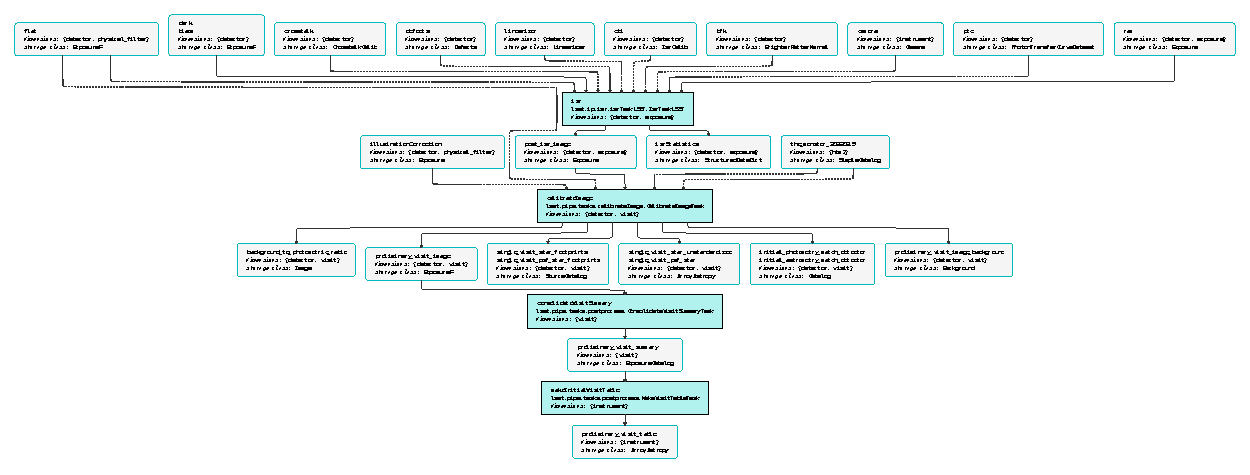
\includegraphics[width=\textwidth]{figures/pipe_viz_comcam_subset.pdf}
    \caption{
        Example pipeline visualization of four selected tasks from the \texttt{LSSTComCam/DRP-v2.yaml} pipeline in the Mermaid format.
        The diagram illustrates the flow of datasets between tasks, with dashed lines indicating prerequisite inputs.
        This visualization helps validate task dependencies and the expected sequence of execution.
    }
    \label{fig:pipe_viz}
\end{figure*}

